% !TEX root = ../thesis.tex

\chapter{Analýza}

\section{Analýza potenciálnych počítačových hier}
Bližšie si pozrieme kandidátov hier na základe možností dát, produktivity, veľkosti ich publika a investovaných fondov do tipovania.

\subsection{Counter-Strike: Global Offensive}
Hra s priemerným publikom viac ako 500 000 hráčov každý deň, publikovaná v roku 2012. Práve prebieha svetový šampionát vo Švédsku s výherným rozpočtom 2 miliónov dolárov. Veľkou časťou tejto hry je verejne dostupný trh s predmetmi získateľnými iba cez túto hru. Tieto predmety majú na podobnom základe ako NFT´s peňažnú hodnotu a poskytujú hráčom vsadiť cez tretie strany na výhercov konkrétnych zápasov, čo viacnásobne zväčšuje tipovací trh. Problémom pri FPS hrách je ale určenie potrebných dát na predpoveď. Výsledok má príliš veľa variácií, kde len milimetre rozhodujú o úplnej zmene priebehu. Dalo by sa určiť víťaza na základe predošlých stretnutí daných dvoch tímov, no tímy sú veľmi ovplyvnené zmenami hráčov, ktoré môžu úplne zmeniť tímovú atmosféru a dáta z predošlých hier sú nepotrebné.
 \subsubsection{Predpovede počas zápasu}
 Jedna hra sa delí na 30 kôl. Prvý tím ktorý dosiahne 16 bodov, vyhráva. Počas kola už firma Valve, tvorca tejto hry, ukázala ich prieskumy a ukazuje, aká je šanca, že daný tím vyhraje kolo na základe miliárd kôl z predchádzajúcich hier. Percentá sa menia podľa počtu živých hráčov, počtu peňazí, mapy, strany a položenia bomby. Za túto funkciu som musel zaplatiť 0,85 eur za mesiac.
  \subsubsection{Predstavenie podobných prístupov}
  Nasledujúce obrázky sú z pozorovania podobných prístupov.
 \begin{figure}
 
 	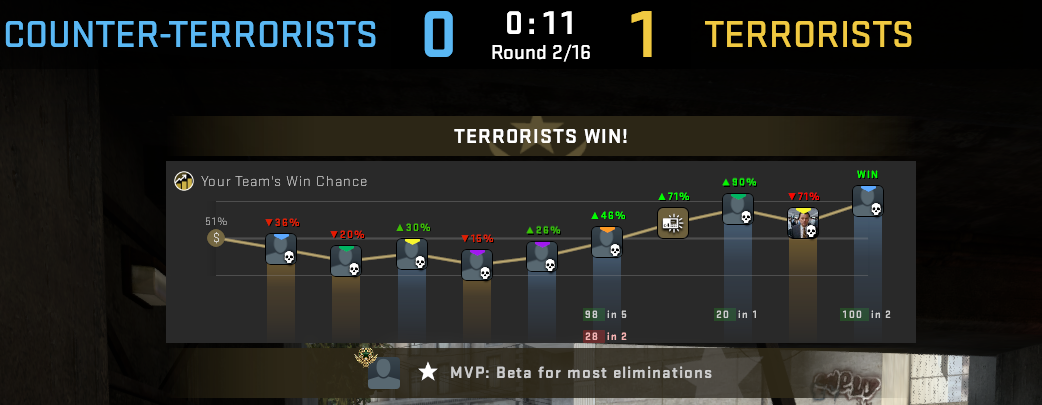
\includegraphics[width=.9\textwidth]{figures/jednanula}
 	\centering
 	\caption{\LaTeX{} Na začiatku môžeme vidieť 51 percentnú pravdepodobnosť na výhru, pri prvom úmrtí nášho spoluhráča šanca klesla na 36 percent, pri druhom až na 20, ale pri zabití nepriateľa šanca stúpla na 30 percent.  \label{jednanula}}
 \end{figure}

  \begin{figure}
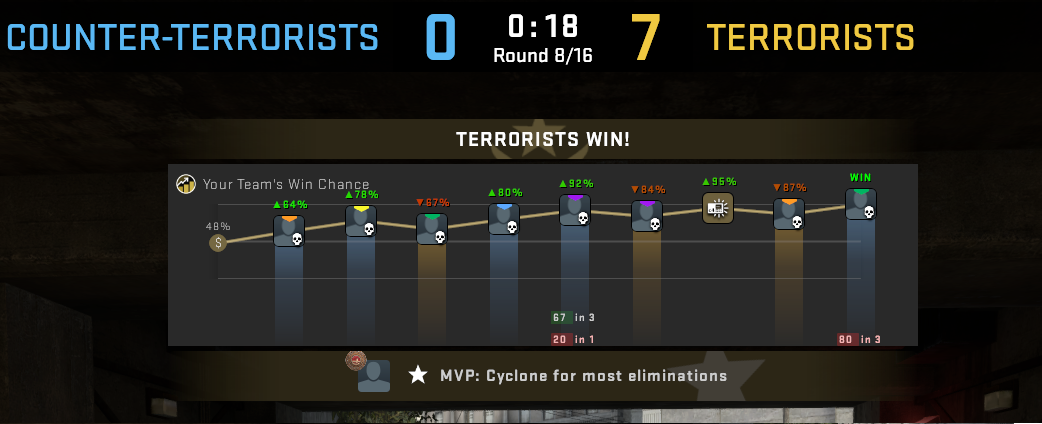
\includegraphics[width=.9\textwidth]{figures/sedemnula}
\centering
\caption{\LaTeX{} Vieme vydedukovať, že čím je šanca na výhru vyššia, tým sa šanca na úmrtie spoluhráča takisto zmenšuje. 
\label{sedemnula}}
\end{figure}
\begin{figure}
	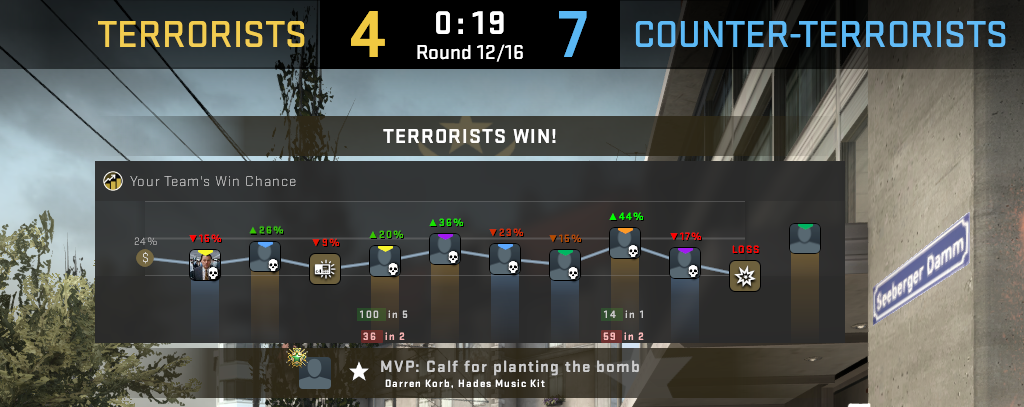
\includegraphics[width=.9\textwidth]{figures/sedemstyri}
	\centering
	\caption{\LaTeX{} Hneď prvé percentu je veľmi nízke, len 24 percent, a to kvôli horšiemu vybaveniu/peňažnej situácie nášho tímu.
		\label{sedemstyri}}
\end{figure}
\begin{figure}
	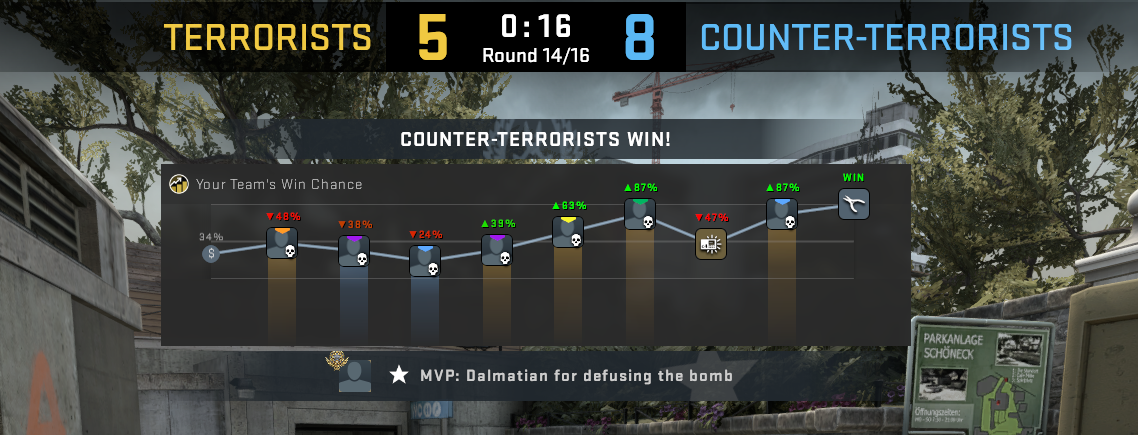
\includegraphics[width=.9\textwidth]{figures/osempat}
	\centering
	\caption{\LaTeX{} Z prvého prechodu si môžete všimnúť stúpnutie šance z 34 na 48 percent, aj keď bol zabitý jeden z našich spoluhráčov. 
		\label{osempat}}
\end{figure}

 \subsubsection{Vyhodnotenie Counter-Strike: Global Offensive}
 Vyhrávajúci tím a zmeny je možné vidieť počas celého daného kola, ale stávky sa berú pred začatím zápasu.
 
Berúc do úvahy potenciál a veľkosť stávkového trhu nie je aktuálne reálne nájsť spôsob predpovedania, a to kvôli kvantám premenných.

\subsection{Dota 2}
Dota je jednou z dvoch najznámejších MOBA hier na svete, s priemerným počtom hráčov viac ako 400 tisíc. Podobne ako Counter-Strike má predmety a verejný trh. Na druhej strane výherný rozpočet sa s ním nedá porovnať, pretože tento rok prekonal 40 miliónov. Umelá inteligencia tejto hre tiež nie je vzdialená. Počítačom sa podarilo nadľudsky zdokonaliť sa a v uzavretých podmienkach porazili aj najlepších ľudských hráčov na svete. Stávkovanie na ľudské tímy je ale iná vec. Dáta sú pri Dote celkom jasné a je možné ich čerpať z OpenDota API na stránke : https://docs.opendota.com/.

\subsection{League of Legends}
Liga Legiend je najrozšírenejšia MOBA hra na svete s viac ako 3 miliónmi každodenných používateľov a viac ako 100 miliónmi mesačných použivateľov. Riot games má podobne ako Dota verejne dostupné informácie pre developerov na stránke : https://developer.riotgames.com/ 

\section{Analýza dostupných spracovaní dát}
\subsection{Supervised learning}
\subsection{Reinforcement learning}
